\section{Modulation}
\todo{Woche 5 - 18.10.21}
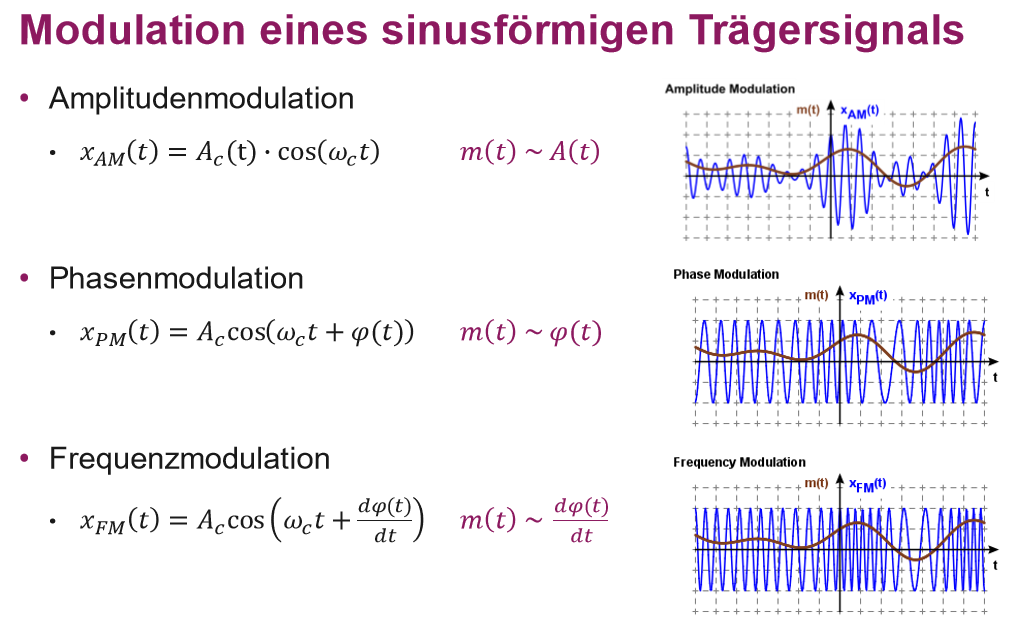
\includegraphics[width=\columnwidth]{Images/screenshot005}

\subsection{Basisbanddarstellung}
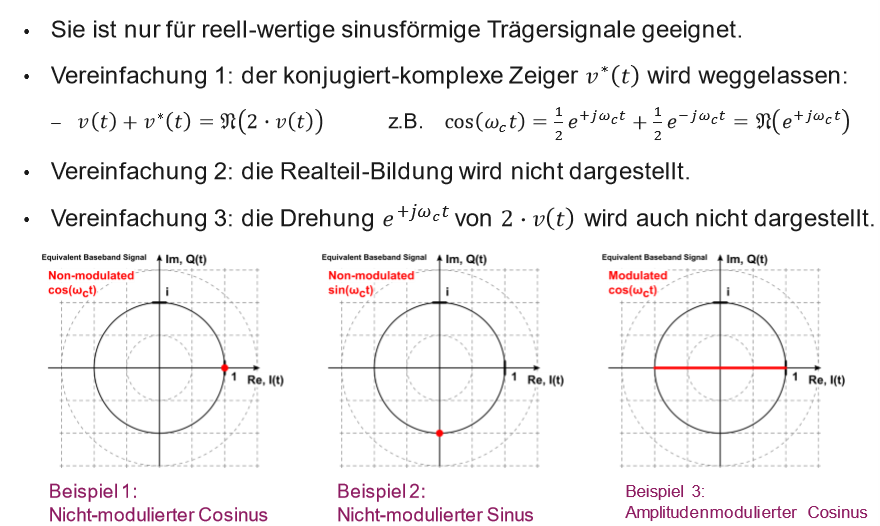
\includegraphics[width=\columnwidth]{Images/screenshot007}


\todo{Woche 7 - 8.11.21\\
	Folgende Spektren zu jeweiligen Kapitel hinzufügen:\\
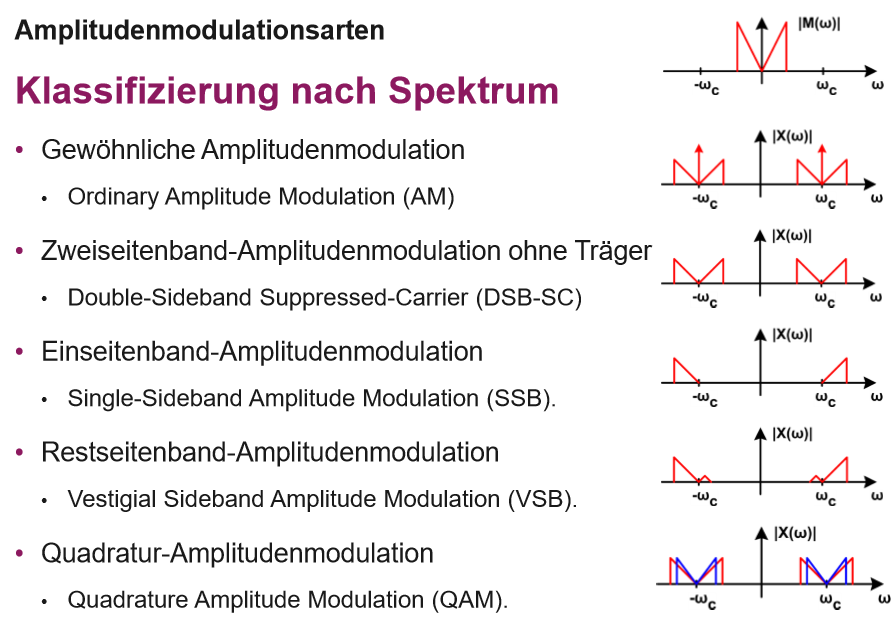
\includegraphics[width=\columnwidth]{Images/klassiefizierung}}


\subsection{AM}
Amplitudentmodulation
\[
X_{AM}(t) = A_c (1 + \mu \cdot m_n(t))\cos(\omega_ct) \]

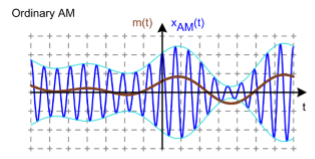
\includegraphics[width=0.5\columnwidth]{Images/am}

\subsubsection{DSB-SC}
Double-sideband suppressed-carrier\\

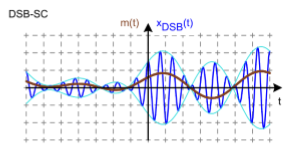
\includegraphics[width=0.5\columnwidth]{Images/dsb_sc}

Im unterschied zu AM kein DC Anteil (Dirac-Stoss) und gesammte Leistungseffizient in Seitenbändern.
\[x_{DSB}(t) = A_c \cdot m_n(t) \cdot cos(\omega_ct)\]

\subsubsection{SSB}
Single-Sideband modulation\\
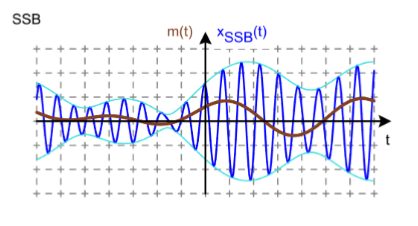
\includegraphics[width=0.5\columnwidth]{Images/ssb}

Wenn Nachrichtensignal $m_n$ Reellwertig ist, dann kann die Negative Frequenzachse weggelassen werden, da diese Konjugiert-Komplex sein müssen. Wobei $\hat{m}_n$ die Hilbert-Transformierte (Frequenz um 90° verschoben) von dem Nachrichtensignal ist.

\[X_{SSB} = A_c \cdot m_n(t) \cdot \cos(\omega_ct) \mp A_c\cdot \hat{m}_n\cdot \sin(\omega_ct)\]

\subsubsection{VSB}
Restseitenband-Amplidudenmodulation\\
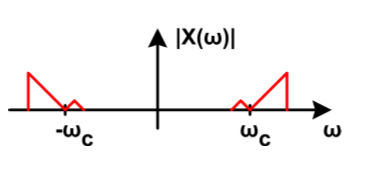
\includegraphics[width=0.5\columnwidth]{Images/vsb}

Eine Seitenband wird komplett, das zweite mit reduzierter Bandbreite Übertragen. Kompromisslösung zwischen SSB und DSB-SC.

\subsubsection{QAM}
Quadraturamplitudenmodulation\\
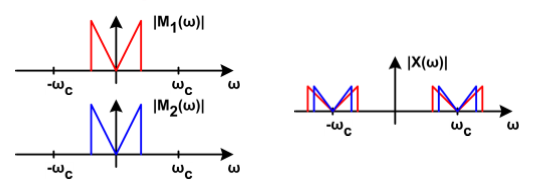
\includegraphics[width=0.5\columnwidth]{Images/qam}

Zwei komplett unabhängige (aber orthogonal zueinander) modulierte DSB-SC Signale sind überlagert.


\subsection{Phasenmodulation}
\todo{Woche 9 - 15.11.21}
Die Phasenmodulation im Zeitbereich wobei $k_p$ die Phasenhubkonstante in [rad] ist.
\[
x_{PM}(t) = A_c\cdot \cos(\omega_ct + \varphi(t)) \qquad \varphi(t) = k_p\cdot m(t)
\]

\subsubsection{Momentanfrequenz}
\todo{
	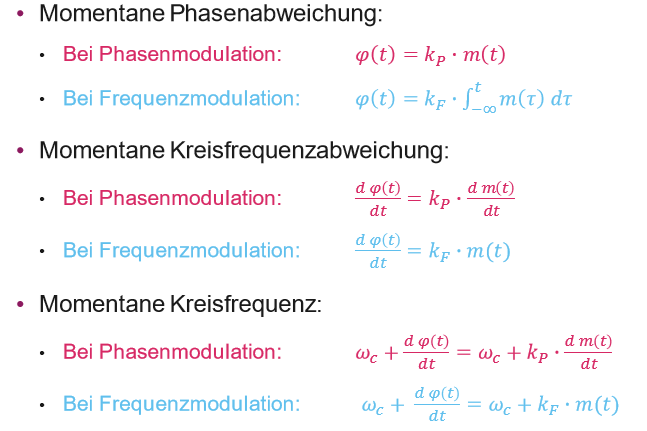
\includegraphics[width=\columnwidth]{Images/screenshot008}
}
Momentanfrequenz $\omega_i(t)$ bei Phasen-und Frequenzmodulation ist die Ableitung des Argumentes $\theta$ vom Trägersignal $s$.\\ \textbf{Beispiel }$s = 10\cos(\underbrace{200\pi t + \frac{\pi}{3}}_\theta) \xrightarrow{\omega_i(t) = \frac{d\theta}{dt}}  2\pi \cdot 100$

\subsubsection{Kleinhub-Winkelmodulation}
Narrowband Angle Modulation für $\varphi(t) < 0.2rad ~12^\circ$. Dies ist aber für AM uninteressant, da die Leistungseffizienz sehr schlecht ist.
\todo{Woche 10}
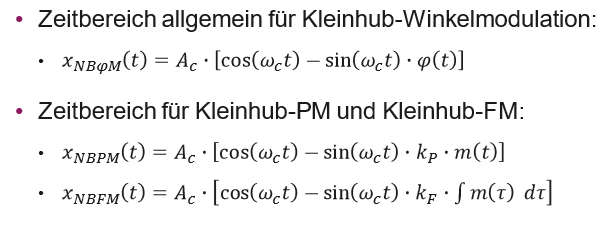
\includegraphics[width=\columnwidth]{Images/screenshot009}

\subsection{Besselfunktion}
\[
x_{ST\varphi M}(t) = A_c \cos(\omega_ct+\beta\sin(\omega_mt)) = A_c \Re[e^{j\omega_ct} \cdot e^{j\beta\sin(\omega_mt)}]
\]
\todo{Woche 10}
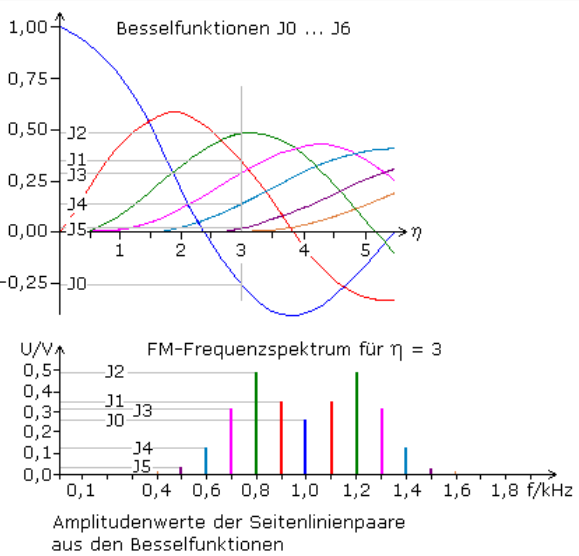
\includegraphics[width=\columnwidth]{Images/besselfunktion}
Maximaler Phasenhub $\max(\varphi(t)) = \beta = k_p\cdot A_m$. 

\subsection{Carson Bandbreite}
\todo{Woche 10}
Die Bandbreite eines Einton-Signals kann Abgeschätzt werden mit Carson:
\begin{align*}
	B_{ST\varphi M} = 2(\beta + 1)\cdot\frac{\omega_m}{2\pi} \\
	B_{PM} = 2(k_pA_m+1)\cdot\frac{\omega_m}{2\pi} \qquad \beta = k_p A_m \\
	B_{FM} = 2\cdot\frac{\omega_mA_m+\omega_m}{2\pi} \qquad \beta = \frac{k_p A_m}{\omega_m}
\end{align*}
Die maximale Frequenzabweichung $B = 2(\Delta f + f_m)$ und das Hubverhältnis $D = \frac{\Delta f}{B}$ 

\textbf{Beispiel:}\\
\begin{align*}
	x(t) &= \underbrace{10}_{A_c}\cos(\underbrace{2\pi10^8}_{\omega_c}t+\underbrace{200}_{\beta}\cos(\underbrace{2\pi10^3}_{\omega_m}t)) \\
	\xrightarrow{\text{W.mod}} B_{ST\varphi M} &= 2(200+1)\cdot 2\pi 10^3 / 2 \pi = 402kHz
\end{align*}


\subsection{Frequenzmodulation}
\todo{Eintonwinkelmodulation}
\todo{Woche 9 - 15.11.21}
Die Frequenzmodulation im Zeitbereich wobei $k_F$ die Frequenzhubkonstante in [rad/s] ist.
\begin{align*}
	x_{FM} = A_c\cdot\cos(\omega_ct + \varphi(t)) \qquad \frac{d\varphi(t)}{dt} &= k_F\cdot m(t) \\
	\varphi(t) &= k_F\int_{-\infty}^{t}m(\tau)d\tau
\end{align*}